\chapter{Ekstrema swobodne i wypukłość}
\label{ma2:ch:free-extrema-convexity}

W tym rozdziale $E$ oznacza rzeczywistą przestrzeń Banacha,
$U\subset E$ zbiór otwarty, a $f:U\to\R$ funkcję skalarną.
Wyniki o pochodnych z rozdziałów 13--16 zastosujemy do
badania ekstremów. Rozróżnimy dodatnią określoność formy
kwadratowej od jej jednostajnej dodatniej określoności:
różnica ta jest istotna w nieskończonym wymiarze.
Ekstrema przy dodatkowych więzach omówimy osobno.

\section{Warunki lokalne}

\begin{definicja}[Ekstrema lokalne i punkty stacjonarne]
\label{ma2:def:free-extrema}
Punkt $p\in U$ jest minimum lokalnym funkcji $f$, jeżeli
istnieje $r>0$ takie, że $B(p,r)\subset U$ oraz
$f(p+h)\ge f(p)$ dla $\|h\|<r$. Minimum jest ścisłe,
jeżeli nierówność jest ostra dla $0<\|h\|<r$.
Maksimum definiujemy przez odwrócenie nierówności.
Ekstremum globalne oznacza odpowiednią nierówność na całym $U$.
Jeżeli istnieje pochodna Frécheta $Df(p)$ i $Df(p)=0$,
punkt $p$ nazywamy stacjonarnym.
\end{definicja}

\begin{twierdzenie}[Warunki konieczne]
\label{ma2:thm:extremum-necessary}
Jeżeli $p$ jest minimum lokalnym i istnieje $Df(p)$,
to $Df(p)=0$. Jeżeli ponadto istnieje druga iterowana
pochodna Frécheta $D^2f(p)$, to
\[
 D^2f(p)[h,h]\ge0\qquad(h\in E).
\]
Dla maksimum otrzymujemy $Df(p)=0$ oraz
$D^2f(p)[h,h]\le0$.
\end{twierdzenie}
\begin{proof}
Ustalmy $h\in E$. Dla $h=0$ obie tezy wynikają
z liniowości i dwuliniowości. Dla $h\ne0$ wybieramy
$r>0$ z definicji minimum i rozpatrujemy
$\gamma(t)=f(p+th)$ dla $|t|<r/\|h\|$.
Z definicji pochodnej
\[
 \gamma(t)-\gamma(0)=tDf(p)h+o(|t|).
\]
Dla $t>0$ iloraz przyrostu przez $t$ jest nieujemny,
dla $t<0$ jest niedodatni. Obie granice są równe
$Df(p)h$, więc $Df(p)h=0$. Dowolność $h$ daje
$Df(p)=0$.

Jeżeli istnieje $D^2f(p)$, wzór Taylora z resztą Peana
(twierdzenie \ref{ma2:thm:taylor-peano}) daje
\[
 0\le f(p+th)-f(p)=\tfrac12t^2D^2f(p)[h,h]+o(t^2)
\]
dla dostatecznie małych $t$. Dzieląc przez $t^2/2$
dla $t\ne0$ i przechodząc do granicy, dostajemy
drugą nierówność. Dla maksimum stosujemy wynik do $-f$.
\end{proof}
Dla funkcji klasy $C^2$ warunki te są także częścią
\atlasref{FA-15::prop:extremum15}{FA-15: kryteria minimum lokalnego}.
Powyższy argument pokazuje, że do warunków punktowych
nie potrzeba ciągłości drugiej pochodnej w otoczeniu.

\begin{definicja}[Określoność formy kwadratowej]
\label{ma2:def:quadratic-definiteness}
Niech $B:E\times E\to\R$ będzie ciągłą symetryczną formą
dwuliniową, a $q(h)=B(h,h)$.
Forma jest dodatnio półokreślona, gdy $q(h)\ge0$
dla każdego $h$, oraz dodatnio określona, gdy
$q(h)>0$ dla każdego $h\ne0$.
Jest jednostajnie dodatnio określona, jeżeli istnieje
$c>0$ takie, że $q(h)\ge c\|h\|^2$ dla każdego $h$.
Określoność ujemną definiujemy przez zastosowanie tych
warunków do $-q$. Forma jest nieokreślona, jeżeli
przyjmuje zarówno wartości dodatnie, jak i ujemne.
\end{definicja}

\begin{twierdzenie}[Warunek dostateczny i wzrost kwadratowy]
\label{ma2:thm:extremum-sufficient}
Niech $Df(p)=0$ i niech istnieje $D^2f(p)$.
Jeżeli dla pewnego $c>0$ mamy
$D^2f(p)[h,h]\ge c\|h\|^2$ dla wszystkich $h\in E$,
to istnieje $r>0$ takie, że $B(p,r)\subset U$ i
\[
 f(p+h)\ge f(p)+\tfrac c4\|h\|^2
 \qquad(\|h\|<r).
\]
W szczególności $p$ jest ścisłym minimum lokalnym.
Jeżeli $D^2f(p)[h,h]\le -c\|h\|^2$, otrzymujemy
ścisłe maksimum i oszacowanie z przeciwnym znakiem.
Odwrotnie, jeśli istnieje $D^2f(p)$ i
$f(p+h)\ge f(p)+\kappa\|h\|^2$ w otoczeniu $p$
dla pewnego $\kappa>0$, to $Df(p)=0$ oraz
$D^2f(p)[h,h]\ge2\kappa\|h\|^2$ dla każdego $h$.
\end{twierdzenie}
\begin{proof}
W przypadku $E=\{0\}$ wszystkie nierówności dotyczą
wyłącznie $h=0$, a warunek ścisłości jest pusty.
Niech $E\ne\{0\}$. Ze wzoru Taylora z resztą Peana
mamy
\[
 f(p+h)-f(p)=\tfrac12 D^2f(p)[h,h]+R(h),
 \qquad R(h)=o(\|h\|^2).
\]
Wybieramy $r>0$, zmniejszając je tak, aby kula należała
do $U$ i $|R(h)|\le(c/4)\|h\|^2$ dla $0<\|h\|<r$.
Ponieważ $R(0)=0$, oszacowanie obowiązuje także dla $h=0$.
Stąd
\[
 f(p+h)-f(p)\ge \tfrac c2\|h\|^2-\tfrac c4\|h\|^2
 =\tfrac c4\|h\|^2.
\]
Maksimum otrzymujemy stosując to samo do $-f$.
W kierunku odwrotnym założenie daje minimum lokalne,
więc twierdzenie \ref{ma2:thm:extremum-necessary}
zapewnia $Df(p)=0$. Dla ustalonego $v\ne0$
podstawiamy $h=tv$ do nierówności i wzoru Taylora.
Po podzieleniu przez $t^2$ i przejściu z $t\to0$
otrzymujemy $\tfrac12 D^2f(p)[v,v]\ge\kappa\|v\|^2$.
Dla $v=0$ zachodzi równość.
\end{proof}
Dowód rozszerza wersję klasy $C^2$ z
\atlasref{FA-15::prop:extremum15}{FA-15}
na istnienie drugiej pochodnej w punkcie.

\begin{stwierdzenie}[Nieokreślona druga pochodna]
\label{ma2:prop:saddle-hessian}
Niech $Df(p)=0$ i niech istnieje $D^2f(p)$.
Jeżeli forma $h\mapsto D^2f(p)[h,h]$ jest nieokreślona,
to w każdym otoczeniu $p$ istnieją punkty $x,y$ takie,
że $f(x)<f(p)<f(y)$. W szczególności $p$ nie jest
ekstremum lokalnym (jest punktem siodłowym w tym sensie).
\end{stwierdzenie}
\begin{proof}
Wybieramy $u,v$ z $D^2f(p)[u,u]>0$ i
$D^2f(p)[v,v]<0$. Oba wektory są niezerowe.
Dla $t\ne0$ dostatecznie małego wzór Taylora daje
\[
 \frac{f(p+tu)-f(p)}{t^2}\longrightarrow
 \tfrac12D^2f(p)[u,u]>0,\qquad
 \frac{f(p+tv)-f(p)}{t^2}\longrightarrow
 \tfrac12D^2f(p)[v,v]<0.
\]
Oba punkty dążą do $p$, należą więc od pewnego momentu
do dowolnego zadanego otoczenia zawartego w $U$.
Granice o przeciwnych znakach zapewniają żądane
nierówności dla dostatecznie małego $t>0$.
\end{proof}

\subsection*{Skończony i nieskończony wymiar}

\begin{stwierdzenie}[Zwartość sfery a określoność]
\label{ma2:prop:finite-positive-coercive}
W niezerowej skończenie wymiarowej przestrzeni
unormowanej $E$ każda ciągła dodatnio określona
forma kwadratowa jest jednostajnie dodatnio określona.
\end{stwierdzenie}
\begin{proof}
Sfera $S=\{h\in E:\|h\|=1\}$ jest niepusta, domknięta
i ograniczona, a w skończonym wymiarze zwarta.
Funkcja $q(h)=B(h,h)$ jest ciągła, więc osiąga na $S$
minimum $c$. Dodatnia określoność daje $c>0$,
ponieważ punkt osiągania minimum ma normę $1$.
Dla $h\ne0$ z jednorodności stopnia drugiego mamy
$q(h)=\|h\|^2q(h/\|h\|)\ge c\|h\|^2$.
Dla $h=0$ zachodzi równość.
\end{proof}

\begin{przyklad}[Dodatnia określoność w nieskończonym wymiarze]
\label{ma2:ex:positive-not-coercive}
Na rzeczywistej przestrzeni Hilberta $H=\ell^2(\N;\R)$
rozważmy
\[
 f(x)=\frac12\sum_{n\ge1}\frac{x_n^2}{n}-\|x\|_2^3.
\]
Z przykładu
\atlasref{FA-15::ex:positive-hessian15}{FA-15: dodatniość bez jednostajności}
wiemy, że $f\in C^2(H,\R)$, $Df(0)=0$ oraz
$D^2f(0)[h,h]=\sum_{n\ge1}h_n^2/n$.
Szereg jest zbieżny, bo jest majoryzowany przez
$\sum_n h_n^2$; dla $h\ne0$ przynajmniej jeden
składnik jest dodatni. Jednak na wektorach jednostkowych
$e_n$ forma przyjmuje wartości $1/n$, więc nie ma
dodatniego jednostajnego ograniczenia dolnego.
Dla $x^{(n)}=e_n/n$ mamy $\|x^{(n)}\|_2=1/n\to0$, a
\[
 f(x^{(n)})=\frac{1}{2n^3}-\frac{1}{n^3}
 =-\frac{1}{2n^3}<0=f(0).
\]
Nie ma zatem minimum lokalnego. W szczególności
nie można zastąpić jednostajnej określoności w
twierdzeniu \ref{ma2:thm:extremum-sufficient} samą
dodatnią określonością.
\end{przyklad}

\section{Macierz Hessego w skończonym wymiarze}

Dla $E=\R^n$, $n\ge1$, jeżeli istnieje $D^2f(p)$,
macierz $H_f(p)$ z definicji \ref{ma2:def:hessian}
jest rzeczywista i symetryczna oraz
\[
 D^2f(p)[h,h]=h^{\mathsf T}H_f(p)h .
\]
Wobec twierdzeń \ref{ma2:thm:extremum-necessary}
i \ref{ma2:thm:extremum-sufficient} oraz
stwierdzenia \ref{ma2:prop:finite-positive-coercive}
dodatnio określona macierz w punkcie stacjonarnym daje
ścisłe minimum, ujemnie określona daje ścisłe maksimum,
a nieokreślona wyklucza oba ekstrema.
Jeżeli macierz jest tylko półokreślona, nie rozstrzyga
to w ogólności o istnieniu ekstremum.

\begin{stwierdzenie}[Kryterium w dwóch zmiennych]
\label{ma2:prop:hessian-two-dim}
Niech $p$ będzie punktem stacjonarnym funkcji
$f:U\subset\R^2\to\R$ z istniejącą $D^2f(p)$ i niech
\[
 H_f(p)=\begin{pmatrix}a&b\\b&c\end{pmatrix},\qquad
 \Delta=ac-b^2.
\]
Jeżeli $\Delta>0$ i $a>0$, punkt jest ścisłym minimum;
jeżeli $\Delta>0$ i $a<0$, jest ścisłym maksimum.
Jeżeli $\Delta<0$, jest punktem siodłowym.
Jeżeli $\Delta=0$, test nie jest w ogólności rozstrzygający.
\end{stwierdzenie}
\begin{proof}
Gdy $a\ne0$, uzupełniamy kwadrat:
\[
 a s^2+2bst+ct^2
 =a(s+(b/a)t)^2+(\Delta/a)t^2.
\]
Dla $\Delta>0$ współczynniki mają ten sam znak
co $a$. Dla $(s,t)\ne(0,0)$ co najmniej jeden kwadrat
jest niezerowy: jeśli $t=0$, to $s\ne0$.
Otrzymujemy określoność odpowiedniego znaku.
Dla $\Delta<0$ i $a\ne0$ wektory $(1,0)$ oraz
$(-b/a,1)$ dają odpowiednio wartości $a$ i $\Delta/a$,
czyli przeciwne znaki. Jeśli $a=0$ i $\Delta<0$,
to $b\ne0$. Dla $t=1$ wartość formy wynosi $2bs+c$;
wybierając $s=(1-c)/(2b)$ oraz $s=(-1-c)/(2b)$
otrzymujemy wartości $1$ i $-1$.
Stosujemy udowodnione kryteria ekstremów.
Nierozstrzygalność przy $\Delta=0$ wykazuje
następny przykład.
\end{proof}

\begin{przyklad}[Zdegenerowana macierz Hessego]
\label{ma2:ex:degenerate-hessian}
Funkcje
\[
 f_+(x,y)=x^2+y^4,\qquad
 f_-(x,y)=x^2-y^4,\qquad f_0(x,y)=x^2
\]
mają w $(0,0)$ zerową pierwszą pochodną oraz tę samą
macierz Hessego $\operatorname{diag}(2,0)$.
Dla $f_+$ suma dwóch nieujemnych składników zeruje
się tylko w początku, więc minimum jest ścisłe.
Dla $f_-$ mamy $f_-(t,0)=t^2>0$ i
$f_-(0,t)=-t^4<0$ przy $t\ne0$, zatem nie ma ekstremum.
Dla $f_0$ minimum nie jest ścisłe, ponieważ
$f_0(0,t)=0$ dla wszystkich $t$. Macierz drugich
pochodnych nie rozróżnia tych trzech sytuacji.
\end{przyklad}

\begin{center}
\begin{minipage}{0.94\linewidth}
\centering
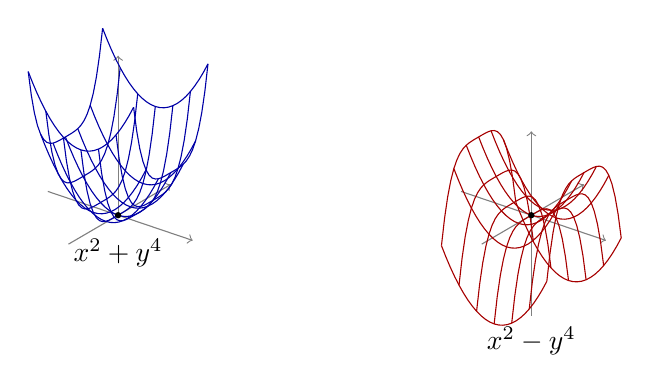
\begin{tikzpicture}[x={(0.68cm,-0.23cm)},y={(0.48cm,0.28cm)},z={(0cm,0.65cm)},scale=0.82]
\begin{scope}[shift={(-3.2cm,0cm)}]
\draw[->,gray] (-1.6,0,0)--(1.7,0,0);
\draw[->,gray] (0,-1.6,0)--(0,1.7,0);
\draw[->,gray] (0,0,0)--(0,0,3.8);
\foreach \a in {-1.2,-0.8,-0.4,0,0.4,0.8,1.2}{
  \draw[blue!65!black,thin] plot[domain=-1.2:1.2,samples=25,variable=\t] (\t,\a,{\t*\t+\a*\a*\a*\a});
  \draw[blue!65!black,thin] plot[domain=-1.2:1.2,samples=25,variable=\t] (\a,\t,{\a*\a+\t*\t*\t*\t});
}
\fill (0,0,0) circle (1.4pt);
\node at (0,0,-0.9) {$x^2+y^4$};
\end{scope}
\begin{scope}[shift={(3.2cm,0cm)}]
\draw[->,gray] (-1.6,0,0)--(1.7,0,0);
\draw[->,gray] (0,-1.6,0)--(0,1.7,0);
\draw[->,gray] (0,0,-2.4)--(0,0,2);
\foreach \a in {-1.2,-0.8,-0.4,0,0.4,0.8,1.2}{
  \draw[red!65!black,thin] plot[domain=-1.2:1.2,samples=25,variable=\t] (\t,\a,{\t*\t-\a*\a*\a*\a});
  \draw[red!65!black,thin] plot[domain=-1.2:1.2,samples=25,variable=\t] (\a,\t,{\a*\a-\t*\t*\t*\t});
}
\fill (0,0,0) circle (1.4pt);
\node at (0,0,-3) {$x^2-y^4$};
\end{scope}
\end{tikzpicture}

\small Dwie funkcje o identycznej macierzy Hessego w początku:
ścisłe minimum (po lewej) i punkt siodłowy (po prawej).
\end{minipage}
\end{center}
